% moved from the main paper to save space
\section{Additional figures}
\label{app:figs}
\begin{figure}[!htbp]
\centering
\figif{fig_pr.pdf}{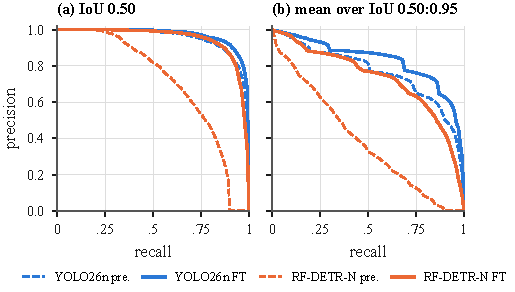
\includegraphics[width=\columnwidth]{figures/fig_pr.pdf}}
\caption{aa1 test precision--recall curves (dashed: COCO-pretrained, solid: fine-tuned).}
\label{fig:pr}
\end{figure}
\begin{figure}[!htbp]
\centering
\figif{fig_selection.pdf}{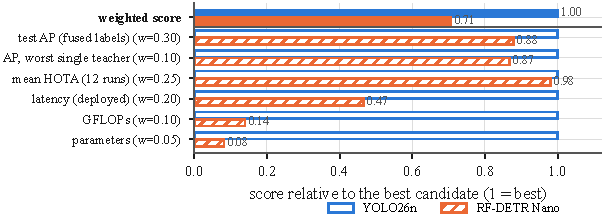
\includegraphics[width=\columnwidth]{figures/fig_selection.pdf}}
\caption{Normalised decision criteria (1 = best candidate) and weighted score.}
\label{fig:sel}
\end{figure}
\begin{figure}[!htbp]
\centering
\figif{fig_edge.pdf}{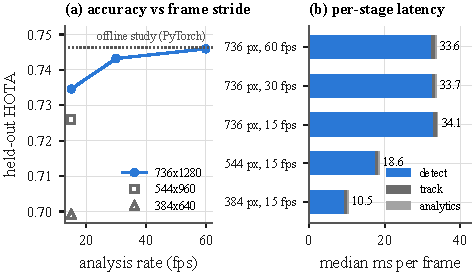
\includegraphics[width=\columnwidth]{figures/fig_edge.pdf}}
\caption{Deployed runtime: (a) held-out HOTA vs.\ analysis rate and input size; (b) median per-stage latency
(desktop CPU ONNX Runtime, not TensorRT).}
\label{fig:edge}
\end{figure}
\section{E2: zero-shot attributes}
\label{app:e2}
\ifHaveVLMETwo
\textbf{E2: zero-shot attributes.} On the held-out campus test tracks, the VLM's zero-shot uniform/gender votes
(three crops per track) are compared with the trained linear probes of Sec.~\ref{sec:campus}. Per track,
dress accuracy is \EtVlmAccUni{} \ci{\EtVlmLoUni}{\EtVlmHiUni} (Wilson CI~\cite{wilson1927}) for the VLM vs.\ \EtProbeAccUni{} for the probe
(coverage \EtVlmCovUni{} vs.\ \EtProbeCovUni), and gender \EtVlmAccGen{} vs.\ \EtProbeAccGen; on the tracks both
answered, an exact McNemar test~\cite{mcnemar1947} gives \EtMcPUni{} and \EtMcPGen. Zero-shot description is thus
competitive with trained probes here.
\fi
